\renewcommand{\leveltopI}{-15cm + \leveltop}
\renewcommand{\leveltopII}{-15cm + \leveltopI}
\renewcommand{\leveltopIII}{-15cm + \leveltopII}
\renewcommand{\leveltopIIII}{-15cm + \leveltopIII}
\renewcommand{\leveltopIIIII}{-15cm + \leveltopIIII}
\renewcommand{\leveltopIIIIII}{-15cm + \leveltopIIIII}
\renewcommand{\leveltopIIIIIII}{-15cm + \leveltopIIIIII}
\begin{tikzpicture}[scale=.2, anchor=south]
\begin{scope}[yshift=\leveltopI cm]
\matrix (line1) [column sep=1cm] {
\node[draw=black, rectangle split,  rectangle split parts=3] (sn0x8412e48){
\begin{tikzpicture}[scale=.2]
\node {4/3};
\end{tikzpicture}
\nodepart{two}
\footnotesize{4.75926}
\nodepart{three}
\footnotesize{$33\:67$}
};
 & 
\\
};
\end{scope}
\begin{scope}[yshift=\leveltopII cm]
\matrix (line2) [column sep=1cm] {
\node[draw=black, rectangle split,  rectangle split parts=3] (sn0x84122b0){
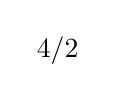
\begin{tikzpicture}[scale=.2]
\node {4/2};
\end{tikzpicture}
\nodepart{two}
\footnotesize{4.58333}
\nodepart{three}
\footnotesize{$33\:67$}
};
 & 
\node[draw=black, rectangle split,  rectangle split parts=3] (sn0x8412b60){
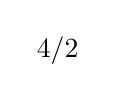
\begin{tikzpicture}[scale=.2]
\node {4/2};
\end{tikzpicture}
\nodepart{two}
\footnotesize{4.34722}
\nodepart{three}
\footnotesize{$33\:33\:33$}
};
 & 
\\
};
\end{scope}
\begin{scope}[yshift=\leveltopIII cm]
\matrix (line3) [column sep=1cm] {
\node[draw=black, rectangle split,  rectangle split parts=3] (sn0x8411a88){
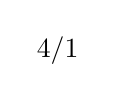
\begin{tikzpicture}[scale=.2]
\node {4/1};
\end{tikzpicture}
\nodepart{two}
\footnotesize{4.5}
\nodepart{three}
\footnotesize{$1$}
};
 & 
\node[draw=black, rectangle split,  rectangle split parts=3] (sn0x8412388){
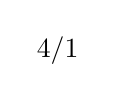
\begin{tikzpicture}[scale=.2]
\node {4/1};
\end{tikzpicture}
\nodepart{two}
\footnotesize{4.125}
\nodepart{three}
\footnotesize{$50\:50$}
};
 & 
\node[draw=black, rectangle split,  rectangle split parts=3] (sn0x8412a88){
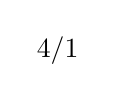
\begin{tikzpicture}[scale=.2]
\node {4/1};
\end{tikzpicture}
\nodepart{two}
\footnotesize{4.25}
\nodepart{three}
\footnotesize{$50\:50$}
};
 & 
\node[draw=black, rectangle split,  rectangle split parts=3] (sn0x8412958){
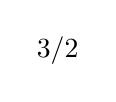
\begin{tikzpicture}[scale=.2]
\node {3/2};
\end{tikzpicture}
\nodepart{two}
\footnotesize{3.66667}
\nodepart{three}
\footnotesize{$67\:33$}
};
 & 
\\
};
\end{scope}
\begin{scope}[yshift=\leveltopIIII cm]
\matrix (line4) [column sep=1cm] {
\node[draw=black, rectangle split,  rectangle split parts=3] (sn0x8411980){
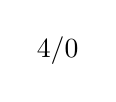
\begin{tikzpicture}[scale=.2]
\node {4/0};
\end{tikzpicture}
\nodepart{two}
\footnotesize{4}
\nodepart{three}
\footnotesize{$1$}
};
 & 
\node[draw=black, rectangle split,  rectangle split parts=3] (sn0x8411fb8){
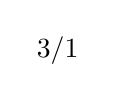
\begin{tikzpicture}[scale=.2]
\node {3/1};
\end{tikzpicture}
\nodepart{two}
\footnotesize{3.25}
\nodepart{three}
\footnotesize{$50\:50$}
};
 & 
\node[draw=black, rectangle split,  rectangle split parts=3] (sn0x8412a10){
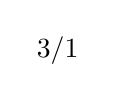
\begin{tikzpicture}[scale=.2]
\node {3/1};
\end{tikzpicture}
\nodepart{two}
\footnotesize{3.5}
\nodepart{three}
\footnotesize{$1$}
};
 & 
\\
};
\end{scope}
\begin{scope}[yshift=\leveltopIIIII cm]
\matrix (line5) [column sep=1cm] {
\node[draw=black, rectangle split,  rectangle split parts=3] (sn0x8411918){
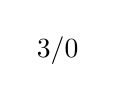
\begin{tikzpicture}[scale=.2]
\node {3/0};
\end{tikzpicture}
\nodepart{two}
\footnotesize{3}
\nodepart{three}
\footnotesize{$1$}
};
 & 
\node[draw=black, rectangle split,  rectangle split parts=3] (sn0x8411e50){
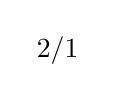
\begin{tikzpicture}[scale=.2]
\node {2/1};
\end{tikzpicture}
\nodepart{two}
\footnotesize{2.5}
\nodepart{three}
\footnotesize{$1$}
};
 & 
\\
};
\end{scope}
\begin{scope}[yshift=\leveltopIIIIII cm]
\matrix (line6) [column sep=1cm] {
\node[draw=black, rectangle split,  rectangle split parts=3] (sn0x8411128){
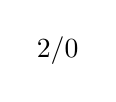
\begin{tikzpicture}[scale=.2]
\node {2/0};
\end{tikzpicture}
\nodepart{two}
\footnotesize{2}
\nodepart{three}
\footnotesize{$1$}
};
 & 
\\
};
\end{scope}
\draw (sn0x8412e48.south) -- (sn0x84122b0.north);
\draw (sn0x8412e48.south) -- (sn0x8412b60.north);
\draw (sn0x84122b0.south) -- (sn0x8411a88.north);
\draw (sn0x84122b0.south) -- (sn0x8412388.north);
\draw (sn0x8412b60.south) -- (sn0x8412a88.north);
\draw (sn0x8412b60.south) -- (sn0x8412388.north);
\draw (sn0x8412b60.south) -- (sn0x8412958.north);
\draw (sn0x8411a88.south) -- (sn0x8411980.north);
\draw (sn0x8412388.south) -- (sn0x8411980.north);
\draw (sn0x8412388.south) -- (sn0x8411fb8.north);
\draw (sn0x8412a88.south) -- (sn0x8411980.north);
\draw (sn0x8412a88.south) -- (sn0x8412a10.north);
\draw (sn0x8412958.south) -- (sn0x8412a10.north);
\draw (sn0x8412958.south) -- (sn0x8411fb8.north);
\draw (sn0x8411980.south) -- (sn0x8411918.north);
\draw (sn0x8411fb8.south) -- (sn0x8411918.north);
\draw (sn0x8411fb8.south) -- (sn0x8411e50.north);
\draw (sn0x8412a10.south) -- (sn0x8411918.north);
\draw (sn0x8411918.south) -- (sn0x8411128.north);
\draw (sn0x8411e50.south) -- (sn0x8411128.north);
\end{tikzpicture}

%%% Local Variables:
%%% TeX-master: "thesis/thesis.tex"
%%% End: 
\renewcommand{\leveltopI}{-15cm + \leveltop}
\renewcommand{\leveltopII}{-15cm + \leveltopI}
\renewcommand{\leveltopIII}{-15cm + \leveltopII}
\renewcommand{\leveltopIIII}{-15cm + \leveltopIII}
\renewcommand{\leveltopIIIII}{-15cm + \leveltopIIII}
\renewcommand{\leveltopIIIIII}{-15cm + \leveltopIIIII}
\renewcommand{\leveltopIIIIIII}{-15cm + \leveltopIIIIII}
\begin{tikzpicture}[scale=.2, anchor=south]
\begin{scope}[yshift=\leveltopI cm]
\matrix (line1) [column sep=1cm] {
\node[draw=black, rectangle split,  rectangle split parts=3] (sn0x8413490){
\begin{tikzpicture}[scale=.2]
\node {4/3};
\end{tikzpicture}
\nodepart{two}
\footnotesize{4.86574}
\nodepart{three}
\footnotesize{$33\:33\:33$}
};
 & 
\\
};
\end{scope}
\begin{scope}[yshift=\leveltopII cm]
\matrix (line2) [column sep=1cm] {
\node[draw=black, rectangle split,  rectangle split parts=3] (sn0x8412878){
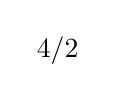
\begin{tikzpicture}[scale=.2]
\node {4/2};
\end{tikzpicture}
\nodepart{two}
\footnotesize{4.66667}
\nodepart{three}
\footnotesize{$33\:67$}
};
 & 
\node[draw=black, rectangle split,  rectangle split parts=3] (sn0x84122b0){
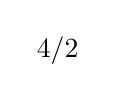
\begin{tikzpicture}[scale=.2]
\node {4/2};
\end{tikzpicture}
\nodepart{two}
\footnotesize{4.58333}
\nodepart{three}
\footnotesize{$33\:67$}
};
 & 
\node[draw=black, rectangle split,  rectangle split parts=3] (sn0x8412b60){
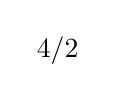
\begin{tikzpicture}[scale=.2]
\node {4/2};
\end{tikzpicture}
\nodepart{two}
\footnotesize{4.34722}
\nodepart{three}
\footnotesize{$33\:33\:33$}
};
 & 
\\
};
\end{scope}
\begin{scope}[yshift=\leveltopIII cm]
\matrix (line3) [column sep=1cm] {
\node[draw=black, rectangle split,  rectangle split parts=3] (sn0x8411a88){
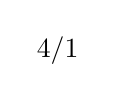
\begin{tikzpicture}[scale=.2]
\node {4/1};
\end{tikzpicture}
\nodepart{two}
\footnotesize{4.5}
\nodepart{three}
\footnotesize{$1$}
};
 & 
\node[draw=black, rectangle split,  rectangle split parts=3] (sn0x8412a88){
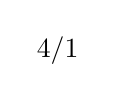
\begin{tikzpicture}[scale=.2]
\node {4/1};
\end{tikzpicture}
\nodepart{two}
\footnotesize{4.25}
\nodepart{three}
\footnotesize{$50\:50$}
};
 & 
\node[draw=black, rectangle split,  rectangle split parts=3] (sn0x8412388){
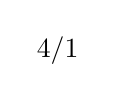
\begin{tikzpicture}[scale=.2]
\node {4/1};
\end{tikzpicture}
\nodepart{two}
\footnotesize{4.125}
\nodepart{three}
\footnotesize{$50\:50$}
};
 & 
\node[draw=black, rectangle split,  rectangle split parts=3] (sn0x8412958){
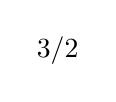
\begin{tikzpicture}[scale=.2]
\node {3/2};
\end{tikzpicture}
\nodepart{two}
\footnotesize{3.66667}
\nodepart{three}
\footnotesize{$33\:67$}
};
 & 
\\
};
\end{scope}
\begin{scope}[yshift=\leveltopIIII cm]
\matrix (line4) [column sep=1cm] {
\node[draw=black, rectangle split,  rectangle split parts=3] (sn0x8411980){
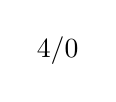
\begin{tikzpicture}[scale=.2]
\node {4/0};
\end{tikzpicture}
\nodepart{two}
\footnotesize{4}
\nodepart{three}
\footnotesize{$1$}
};
 & 
\node[draw=black, rectangle split,  rectangle split parts=3] (sn0x8412a10){
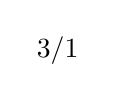
\begin{tikzpicture}[scale=.2]
\node {3/1};
\end{tikzpicture}
\nodepart{two}
\footnotesize{3.5}
\nodepart{three}
\footnotesize{$1$}
};
 & 
\node[draw=black, rectangle split,  rectangle split parts=3] (sn0x8411fb8){
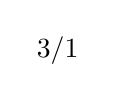
\begin{tikzpicture}[scale=.2]
\node {3/1};
\end{tikzpicture}
\nodepart{two}
\footnotesize{3.25}
\nodepart{three}
\footnotesize{$50\:50$}
};
 & 
\\
};
\end{scope}
\begin{scope}[yshift=\leveltopIIIII cm]
\matrix (line5) [column sep=1cm] {
\node[draw=black, rectangle split,  rectangle split parts=3] (sn0x8411918){
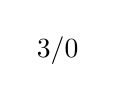
\begin{tikzpicture}[scale=.2]
\node {3/0};
\end{tikzpicture}
\nodepart{two}
\footnotesize{3}
\nodepart{three}
\footnotesize{$1$}
};
 & 
\node[draw=black, rectangle split,  rectangle split parts=3] (sn0x8411e50){
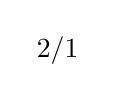
\begin{tikzpicture}[scale=.2]
\node {2/1};
\end{tikzpicture}
\nodepart{two}
\footnotesize{2.5}
\nodepart{three}
\footnotesize{$1$}
};
 & 
\\
};
\end{scope}
\begin{scope}[yshift=\leveltopIIIIII cm]
\matrix (line6) [column sep=1cm] {
\node[draw=black, rectangle split,  rectangle split parts=3] (sn0x8411128){
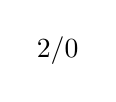
\begin{tikzpicture}[scale=.2]
\node {2/0};
\end{tikzpicture}
\nodepart{two}
\footnotesize{2}
\nodepart{three}
\footnotesize{$1$}
};
 & 
\\
};
\end{scope}
\draw (sn0x8413490.south) -- (sn0x8412878.north);
\draw (sn0x8413490.south) -- (sn0x84122b0.north);
\draw (sn0x8413490.south) -- (sn0x8412b60.north);
\draw (sn0x8412878.south) -- (sn0x8411a88.north);
\draw (sn0x8412878.south) -- (sn0x8412a88.north);
\draw (sn0x84122b0.south) -- (sn0x8411a88.north);
\draw (sn0x84122b0.south) -- (sn0x8412388.north);
\draw (sn0x8412b60.south) -- (sn0x8412a88.north);
\draw (sn0x8412b60.south) -- (sn0x8412388.north);
\draw (sn0x8412b60.south) -- (sn0x8412958.north);
\draw (sn0x8411a88.south) -- (sn0x8411980.north);
\draw (sn0x8412a88.south) -- (sn0x8411980.north);
\draw (sn0x8412a88.south) -- (sn0x8412a10.north);
\draw (sn0x8412388.south) -- (sn0x8411980.north);
\draw (sn0x8412388.south) -- (sn0x8411fb8.north);
\draw (sn0x8412958.south) -- (sn0x8412a10.north);
\draw (sn0x8412958.south) -- (sn0x8411fb8.north);
\draw (sn0x8411980.south) -- (sn0x8411918.north);
\draw (sn0x8412a10.south) -- (sn0x8411918.north);
\draw (sn0x8411fb8.south) -- (sn0x8411918.north);
\draw (sn0x8411fb8.south) -- (sn0x8411e50.north);
\draw (sn0x8411918.south) -- (sn0x8411128.north);
\draw (sn0x8411e50.south) -- (sn0x8411128.north);
\end{tikzpicture}

%%% Local Variables:
%%% TeX-master: "thesis/thesis.tex"
%%% End: 
\renewcommand{\leveltopI}{-15cm + \leveltop}
\renewcommand{\leveltopII}{-15cm + \leveltopI}
\renewcommand{\leveltopIII}{-15cm + \leveltopII}
\renewcommand{\leveltopIIII}{-15cm + \leveltopIII}
\renewcommand{\leveltopIIIII}{-15cm + \leveltopIIII}
\renewcommand{\leveltopIIIIII}{-15cm + \leveltopIIIII}
\renewcommand{\leveltopIIIIIII}{-15cm + \leveltopIIIIII}
\begin{tikzpicture}[scale=.2, anchor=south]
\begin{scope}[yshift=\leveltopI cm]
\matrix (line1) [column sep=1cm] {
\node[draw=black, rectangle split,  rectangle split parts=3] (sn0x84134f8){
\begin{tikzpicture}[scale=.2]
\node {4/3};
\end{tikzpicture}
\nodepart{two}
\footnotesize{4.78704}
\nodepart{three}
\footnotesize{$33\:67$}
};
 & 
\\
};
\end{scope}
\begin{scope}[yshift=\leveltopII cm]
\matrix (line2) [column sep=1cm] {
\node[draw=black, rectangle split,  rectangle split parts=3] (sn0x8412878){
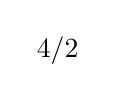
\begin{tikzpicture}[scale=.2]
\node {4/2};
\end{tikzpicture}
\nodepart{two}
\footnotesize{4.66667}
\nodepart{three}
\footnotesize{$33\:67$}
};
 & 
\node[draw=black, rectangle split,  rectangle split parts=3] (sn0x8412b60){
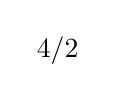
\begin{tikzpicture}[scale=.2]
\node {4/2};
\end{tikzpicture}
\nodepart{two}
\footnotesize{4.34722}
\nodepart{three}
\footnotesize{$33\:33\:33$}
};
 & 
\\
};
\end{scope}
\begin{scope}[yshift=\leveltopIII cm]
\matrix (line3) [column sep=1cm] {
\node[draw=black, rectangle split,  rectangle split parts=3] (sn0x8411a88){
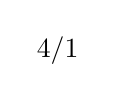
\begin{tikzpicture}[scale=.2]
\node {4/1};
\end{tikzpicture}
\nodepart{two}
\footnotesize{4.5}
\nodepart{three}
\footnotesize{$1$}
};
 & 
\node[draw=black, rectangle split,  rectangle split parts=3] (sn0x8412a88){
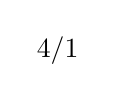
\begin{tikzpicture}[scale=.2]
\node {4/1};
\end{tikzpicture}
\nodepart{two}
\footnotesize{4.25}
\nodepart{three}
\footnotesize{$50\:50$}
};
 & 
\node[draw=black, rectangle split,  rectangle split parts=3] (sn0x8412388){
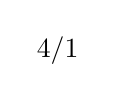
\begin{tikzpicture}[scale=.2]
\node {4/1};
\end{tikzpicture}
\nodepart{two}
\footnotesize{4.125}
\nodepart{three}
\footnotesize{$50\:50$}
};
 & 
\node[draw=black, rectangle split,  rectangle split parts=3] (sn0x8412958){
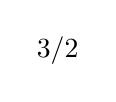
\begin{tikzpicture}[scale=.2]
\node {3/2};
\end{tikzpicture}
\nodepart{two}
\footnotesize{3.66667}
\nodepart{three}
\footnotesize{$33\:67$}
};
 & 
\\
};
\end{scope}
\begin{scope}[yshift=\leveltopIIII cm]
\matrix (line4) [column sep=1cm] {
\node[draw=black, rectangle split,  rectangle split parts=3] (sn0x8411980){
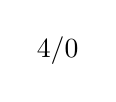
\begin{tikzpicture}[scale=.2]
\node {4/0};
\end{tikzpicture}
\nodepart{two}
\footnotesize{4}
\nodepart{three}
\footnotesize{$1$}
};
 & 
\node[draw=black, rectangle split,  rectangle split parts=3] (sn0x8412a10){
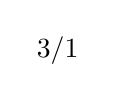
\begin{tikzpicture}[scale=.2]
\node {3/1};
\end{tikzpicture}
\nodepart{two}
\footnotesize{3.5}
\nodepart{three}
\footnotesize{$1$}
};
 & 
\node[draw=black, rectangle split,  rectangle split parts=3] (sn0x8411fb8){
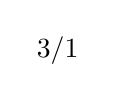
\begin{tikzpicture}[scale=.2]
\node {3/1};
\end{tikzpicture}
\nodepart{two}
\footnotesize{3.25}
\nodepart{three}
\footnotesize{$50\:50$}
};
 & 
\\
};
\end{scope}
\begin{scope}[yshift=\leveltopIIIII cm]
\matrix (line5) [column sep=1cm] {
\node[draw=black, rectangle split,  rectangle split parts=3] (sn0x8411918){
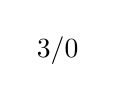
\begin{tikzpicture}[scale=.2]
\node {3/0};
\end{tikzpicture}
\nodepart{two}
\footnotesize{3}
\nodepart{three}
\footnotesize{$1$}
};
 & 
\node[draw=black, rectangle split,  rectangle split parts=3] (sn0x8411e50){
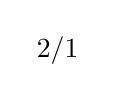
\begin{tikzpicture}[scale=.2]
\node {2/1};
\end{tikzpicture}
\nodepart{two}
\footnotesize{2.5}
\nodepart{three}
\footnotesize{$1$}
};
 & 
\\
};
\end{scope}
\begin{scope}[yshift=\leveltopIIIIII cm]
\matrix (line6) [column sep=1cm] {
\node[draw=black, rectangle split,  rectangle split parts=3] (sn0x8411128){
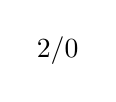
\begin{tikzpicture}[scale=.2]
\node {2/0};
\end{tikzpicture}
\nodepart{two}
\footnotesize{2}
\nodepart{three}
\footnotesize{$1$}
};
 & 
\\
};
\end{scope}
\draw (sn0x84134f8.south) -- (sn0x8412878.north);
\draw (sn0x84134f8.south) -- (sn0x8412b60.north);
\draw (sn0x8412878.south) -- (sn0x8411a88.north);
\draw (sn0x8412878.south) -- (sn0x8412a88.north);
\draw (sn0x8412b60.south) -- (sn0x8412a88.north);
\draw (sn0x8412b60.south) -- (sn0x8412388.north);
\draw (sn0x8412b60.south) -- (sn0x8412958.north);
\draw (sn0x8411a88.south) -- (sn0x8411980.north);
\draw (sn0x8412a88.south) -- (sn0x8411980.north);
\draw (sn0x8412a88.south) -- (sn0x8412a10.north);
\draw (sn0x8412388.south) -- (sn0x8411980.north);
\draw (sn0x8412388.south) -- (sn0x8411fb8.north);
\draw (sn0x8412958.south) -- (sn0x8412a10.north);
\draw (sn0x8412958.south) -- (sn0x8411fb8.north);
\draw (sn0x8411980.south) -- (sn0x8411918.north);
\draw (sn0x8412a10.south) -- (sn0x8411918.north);
\draw (sn0x8411fb8.south) -- (sn0x8411918.north);
\draw (sn0x8411fb8.south) -- (sn0x8411e50.north);
\draw (sn0x8411918.south) -- (sn0x8411128.north);
\draw (sn0x8411e50.south) -- (sn0x8411128.north);
\end{tikzpicture}

%%% Local Variables:
%%% TeX-master: "thesis/thesis.tex"
%%% End: 
